% ****** Start of file apssamp.tex ******
%
%   This file is part of the APS files in the REVTeX 4.1 distribution.
%   Version 4.1r of REVTeX, August 2010
%
%   Copyright (c) 2009, 2010 The American Physical Society.
%
%   See the REVTeX 4 README file for restrictions and more information.
%
% TeX'ing this file requires that you have AMS-LaTeX 2.0 installed
% as well as the rest of the prerequisites for REVTeX 4.1
%
% See the REVTeX 4 README file
% It also requires running BibTeX. The commands are as follows:
%
%  1)  latex apssamp.tex
%  2)  bibtex apssamp
%  3)  latex apssamp.tex
%  4)  latex apssamp.tex
%
\documentclass[%
 reprint,
%superscriptaddress,
%groupedaddress,
%unsortedaddress,
%runinaddress,
%frontmatterverbose, 
%preprint,
%showpacs,preprintnumbers,
%nofootinbib,
%nobibnotes,
%bibnotes,
 amsmath,amssymb,
 aps,
%pra,
%prb,
%rmp,
%prstab,
%prstper,
%floatfix,
]{revtex4-1}

\usepackage{graphicx}% Include figure files
\usepackage{dcolumn}% Align table columns on decimal point
\usepackage{bm}% bold math
\usepackage{color}
%\usepackage{hyperref}% add hypertext capabilities
%\usepackage[mathlines]{lineno}% Enable numbering of text and display math
%\linenumbers\relax % Commence numbering lines

%\usepackage[showframe,%Uncomment any one of the following lines to test 
%%scale=0.7, marginratio={1:1, 2:3}, ignoreall,% default settings
%%text={7in,10in},centering,
%%margin=1.5in,
%%total={6.5in,8.75in}, top=1.2in, left=0.9in, includefoot,
%%height=10in,a5paper,hmargin={3cm,0.8in},
%]{geometry}

%%%%%%%%%%%%%%%%%%%%%%%%%%%%%%%%%%%%%%%%%%%%%%%%%%%%%%%%%%%%%%%%%%%%%
%  needed macros:

%new commands:

%\newcommand{\juan}[1]{\textcolor{blue}{{#1}}}
%\newcommand{\keisuke}[1]{\textcolor{magenta}{#1}}
%\newcommand{\jim}[1]{\textcolor{green}{#1}}
%\newcommand{\todo}[1]{\textcolor{red}{{#1}}}
\newcommand{\juan}[1]{\textcolor{black}{{#1}}}
\newcommand{\keisuke}[1]{\textcolor{black}{#1}}
\newcommand{\jim}[1]{\textcolor{black}{#1}}
\newcommand{\todo}[1]{\textcolor{black}{{#1}}}
%text macros:

\def\etal{{\it et al.}}
\def\etc{{\it etc.}}
\def\eg{{\it e.g.}}
\def\Tab#1{Tab.~\ref{#1}}
\def\Fig#1{Fig.~\ref{#1}}
\def\Figs#1{Figs.~\ref{#1}}
\def\Eq#1{Eq.~(\ref{#1})}
\def\Ref#1{Ref.~\cite{#1}}
\def\Refs#1{Refs.~\cite{#1}}



% math mode macros:

\def\ee{e^+e^-} 

%%%%%%%%%%%%%%%%%%%%%%%%%%%%%%%%%%%%%%%%%%%%%%%%%%%%%%%%%%%%%%%%%%%%%%


\begin{document}

\preprint{LCCPEB---}

\title{The International Linear Collider \\ A Global Project}% Force line breaks with \\
\thanks{Version 1.3}%

\author{Jim Brau}
% \altaffiliation[Also at ]{Physics Department, XYZ University.}%Lines break automatically or can be forced with \\
\author{et.al.}%
 \email{Second.Author@institution.edu}
\affiliation{%
 Authors' institution and/or address\\
% This line break forced with \textbackslash\textbackslash
}%

\collaboration{Linear Collider Collaboration}%\noaffiliation

\date{\today}% It is always \today, today,
             %  but any date may be explicitly specified

\begin{abstract}
Input from the International Linear Collider community for the European Strategy Update 

\end{abstract}

\pacs{Valid PACS appear here}% PACS, the Physics and Astronomy
                             % Classification Scheme.
%\keywords{Suggested keywords}%Use showkeys class option if keyword
%display desired
\maketitle

%\tableofcontents

\section{\label{sec:intro}Introduction}

\todo{ 1 page - Jim and Juan
 Introduce the ILC250, brief overview of status (technical maturity and TDR, staging, cost analysis, status of political situation) }

\juan{The central issue in particle physics today is the search for new phenomena} needed to address shortcomings of the highly successful Standard Model.  \juan{These new effects can manifest as new particles, new forces or deviations in the predictions of the Standard Model derived from high precision measurements.}
With the discovery of the Higgs boson in 2012 at the Large Hadron Collider,
the Standard Model was completed.  
While theoretically self-consistent, with
no evidence of physics beyond the Standard Model having appeared, a number of issues remain
unaddressed, leaving the Standard Model as an incomplete theory of the fundamental
interactions.  New particles or forces could advance our understanding
of how the physics of the Standard Model fits into a more complete
picture of the nature of the universe.

Among the outstanding questions that are the focus of energy frontier
efforts are the explanation of the apparent mismatch of the scale of
electroweak physics with the Planck scale, or the hierarchy problem.
Why is the Higgs mass as light as it is~?
The Standard Model does not offer any explanation for the evidence for dark matter.
Likewise, gravitation is not included.  These and other issues
motivate intense efforts to \juan{test the consistency} of the Standard Model \juan{to high accuracy}
and \juan{look for} small deviations that would provide clues toward answering such
open questions.

For more than twenty years the worldwide community has been engaged in a research
program developing the technology required to realize a high energy linear collider
to precisely measure electron-positron collisions, contributing to 
answering the critical questions at the energy frontier: such as the hierarchy problem,
the nature of dark matter and even the relationship of gravity.
The effort to design and establish the technology for the linear collider 
culminated in the publication of the Technical Design Report (TDR)
for the International Linear Collider (ILC) in 2013~\cite{Behnke:2013xla}. 
\juan{  The \jim{ILC250} is a $250\,{\mathrm{GeV}}$ (extendable up to $1\,{\mathrm{TeV}}$) linear $e^+e^-$ collider, based on $1.3\,{\mathrm{GHz}}$ superconducting radio-frequency (SCRF) cavities. It is designed to  achieve a luminosity of $1.5\cdot 10^{34}~{\mathrm{cm}}^{-1}{\mathrm{s}}^{-1}$ and provide an integrated luminosity of $350\,{\mathrm{fb}}^{-1}$ in the first four years of running. The electron beam will be polarised to $80\,\%$, and positrons with $30\,\%$ polarization will be provided if the undulator based positron source concept is employed.} The parameters were set by considerations of the physics goal,
with an energy reach designed to likely provide access to the mechanism of 
electroweak symmetry breaking (Higgs or no-Higgs)~\cite{Baer:2013cma}.

\juan{ The collider design is thus the result of nearly twenty years of R\&D. The heart of the ILC, the superconducting cavities, is based on over a decade of pioneering work by the TESLA collaboration in the 1990s. Some other aspects were based on the R\&D carried out for the JLC/GLC and NLC projects, which were based on room-temperature accelerating structures. From 2005 to the publication of the TDR~\cite{Behnke:2013xla} in 2013, the design of the ILC accelerator was conducted as a worldwide international collaboration coordinated by the Global Design Effort (GDE) under a mandate from the International Committee for Future Accelerators (ICFA).
Since then, the Linear Collider Collaboration (LCC) has been coordinating the international activities for both the ILC and CLIC projects, again mandated by ICFA.}

%The ILC presented in the TDR is a 200-500 GeV (extendable to 1 TeV) centre-of-mass 
%high luminosity linear electron-positron collider, based on 1.3 GHz superconducting radio-frequency (SCRF)
%accelerating technology~\cite{Adolphsen:2013kya}. 
%Some relevant parameters are given in Tab.~\ref{tab:ilc-params}.}

Once the mass of the Higgs boson was known, it was established that the
linear collider could begin to address these questions in unique fashion
with an initial center-of-mass energy of 250 GeV \jim{at a cost reduced from the TDR.}
A revised design of the ILC (the ILC250) has been presented~\cite{Evans:2017rvt}
based on the ILC TDR.  This design retains the final focus and beam dump
capability to extend the centre-of-mass energy to \juan{higher energies}.  The cost estimate for ILC250 has 
been developed and presented as well.

Additionally, advances in the theoretical understanding of the impact of precision
measurements of the Higgs boson couplings by ILC250 have increased the understanding
of their sensitivity to physics beyond the Standard Model~\cite{Barklow:2017suo,Fujii:2017vwa}. 

The experimental community has developed the designs for two complementary detectors,
ILD and SiD~\cite{Behnke:2013lya}.  These detectors are designed to optimally address the
ILC physics goals.  They are based on a detector R\&D program that has \juan{as well}
contributed a number of advances in detector capabilities \juan{and applications beyond the ILC}.
An additional key need for the experimental program is the software and computing.

This report summarizes the current status of this effort \juan{describing the physics reach, the technological maturity of the accelerator, detector and software/computing development plus a short discussion on the possible future scenarios to realize the project.} 

\section{\label{sec:phys}Physics}

\todo{  [2 pages - Michael, Christophe, Keisuke, Jenny, Junping] }

The physics case for the construction of the ILC is very strong.   The
most important item in this case is the ability to study the couplings
of the Higgs boson with high precision.  The ILC at 250~GeV \juan{(ILC250)} also
presents many opportunities to discover new particles that go beyond
the capabilities of the LHC.  \juan{The ILC with polarized beams \jim{introduces} additional observables 
which increase the sensitivity to both, to precise physics measurements and to direct searches of new physics}. Finally, the \juan{ILC250} opens the
door to further exploration of $\ee$ reactions at higher energies. 
The ILC physics case is reviewed at greater length in the reference
document~\cite{ILCforESS}. 

The Higgs boson is a necessary yet also mysterious part of the
Standard Model of Particle Physics (SM).    In the SM, the Higgs field
couples to every elementary particle and provides the mass for all
quarks, leptons, and heavy vector bosons.   The LHC has now discovered
the Higgs particle and confirmed the couplings responsible for the
masses of the $W$, $Z$, $t$, $b$, and $\tau$ at the qualitative
level~\cite{LHCHiggssummary}.  However, many mysteries could still be
buried here.   The Higgs couplings are not universal, as the gauge
couplings are, and their pattern (which is also the pattern of lepton
and quark masses) is not explained by the SM.  The basic phenomenon that provides
mass for elementary particles---the spontaneous breaking of the gauge
symmetry $SU(2)\times U(1)$---is not explained, and actually cannot be
explained, by the SM.   The Higgs boson could also couple to new
particles and fields that have no SM gauge interactions and are
otherwise completely inaccessible to observation.  Thus, detailed
examination of the Higgs boson properties should be the next major
goal for particle physics experiements.

Within the SM, the couplings of the Higgs boson are specified now that
the parameters of the model, including the Higgs boson mass, are
known.  Expected improvements in the SM parameters in the 2020's will
allow these couplings to be predicted to the part-per-mille level~\cite{Lepage:2014fla}.
Models of new physics correct  these predictions.   These corrections
are predicted to be small, at the 10\% level or below, but they can
be visible to precision experiments.   Most importantly, different
classes of models affect the various Higgs couplings differently, so that
systematic measurement of the Higgs couplings can reveal clues to the
nature of the new interactions.   The precision study of the Higgs
boson interactions then provides a new method both to {\it discover}  the
presence of physics beyond the SM and to {\it learn}  about its nature.

The couplings of the Higgs boson are now being studied at the LHC, but
it is unlikely that the LHC experiments will be able to reach the
level of precision required for sensitivity to new physics models. 
It is important to remember that the goal of
precision Higgs measurement is not to confirm the SM at a given level
of accuracy but rather to discover robust deviations from the SM
pattern that are signals of new physics.   For all Higgs decay modes in which the
Higgs boson does not appear as a resonance (that is, for all decays
except those to 
$\gamma\gamma$ and $4\ell$), Higgs boson event samples at the LHC are dominated
by SM background processes.  Complex selections are needed to make the
Higgs boson component visible. A few percent modelling uncertainty in
the estimation of the SM backgrounds
 destroys the ability to measure Higgs couplings at the 5\%
level.  Further, since this uncertainty is a systematic error, it will
always leave the question of whether deviations from the SM have truly
been observed.

What is needed for a precision Higgs boson measurement program
is a new experimental method in which all individual Higgs boson decay events
are manifest and can be studied in detail.   This is provided by the reaction
$\ee\to Zh$ at 250~GeV in the center of mass. With small and precisely 
calculable SM backgrounds, any $Z$ boson observed with a lab energy 
of 110~GeV is recoiling against a Higgs boson.   Selecting such events 
gives the profile of Higgs boson decays, in SM leptonic and hadron modes 
and even in invisible or partially visible exotic modes. 

Further, since the cross section for Higgs production can be measured
without measuring any property of the Higgs boson, the scale of Higgs
couplings can be determined and the individual couplings can be
absolutely normalized.  Each individual coupling can be compared to
its SM prediction.

In the description of new physics by an  $SU(2)\times U(1)$-invariant
effective field theory (EFT), new physics effects on the  Higgs boson
couplings to $W$ and $Z$ are related to new physics effects on
precision electroweak observables and in $\ee\to W^+W^-$.   This
latter reaction can also be studied to high precision at an $\ee$
collider.  Beam polarization at the ILC is an especially powerful tool
to separate the contributions of different EFT
coefficients. In \cite{Barklow:2017suo}, it is shown that {\it all}
relevant EFT coefficients can be fit {\it simultaneously} from the multiple
observables available at the ILC, giving a 
determination of Higgs boson couplings that is as
model-independent as the EFT description itself. 
 This analysis is reviewed in detail in \cite{ILCforESS}. 
For the nominal \juan{ILC250} program, we predict that the Higgs
coupling to $b$ quarks will be measured to 1\% accuracy and the
couplings to $W$ and $Z$ to 0.7\% accuracy.  The spectrum of  expected
measurements is shown in \Fig{fig:Higgssummary}.  Note that the 
discovery of any anomaly at 250~GeV can be confirmed in running \juan{at higher energies (\eg 500~GeV) by}
using additional reactions  such as $WW$ fusion production of the
Higgs boson.   Measurements at this level can discover---and distinguish---models of new physics over a
wide space of possibilities, even for models in which the predicted new
particles are too heavy to be discovered at the LHC~\cite{Barklow:2017suo}. \juan{Having the ability to 
use polarized beams plays an important role in order to achieve these goals.}

%%%%%%%%%%%%%%%%
\begin{figure}
\begin{center}
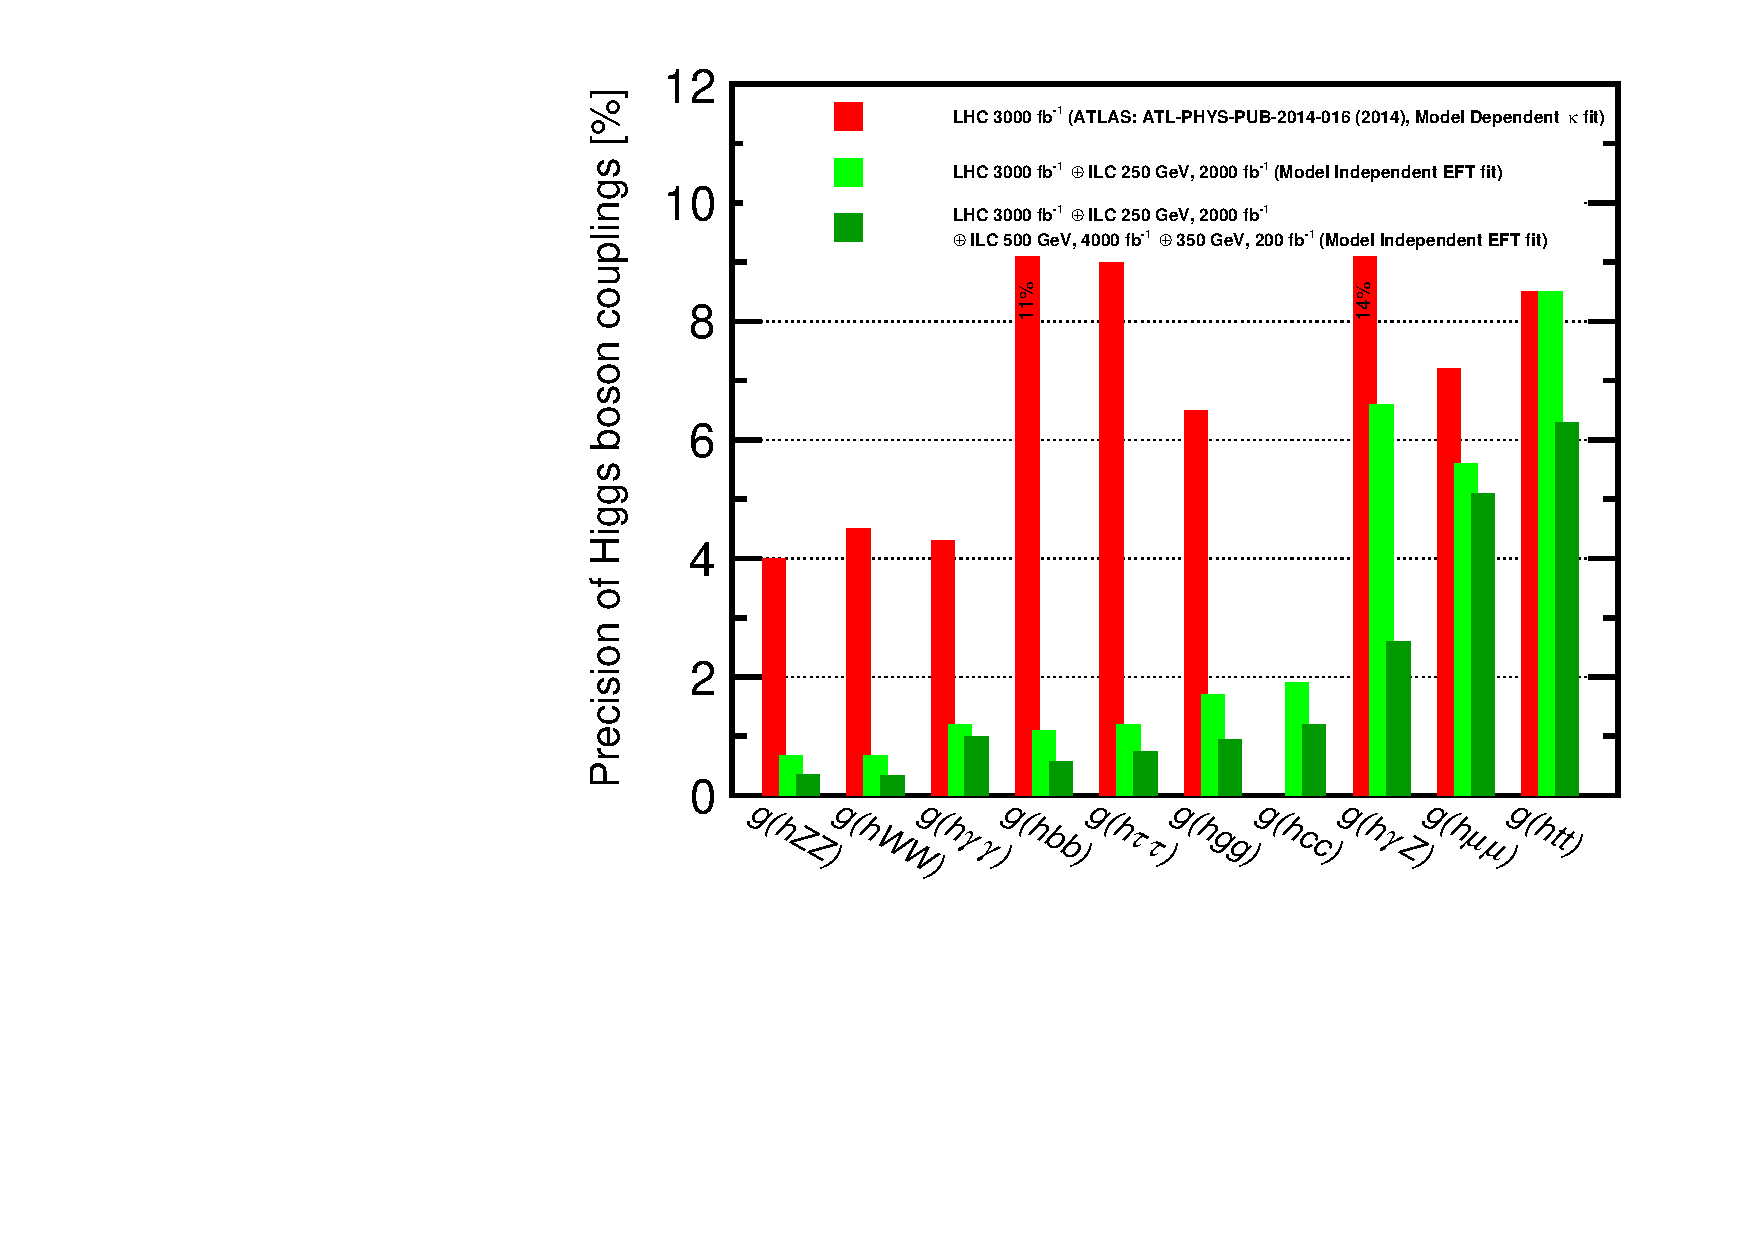
\includegraphics[width=0.95\hsize]{figures/DeltaH_EFT.pdf}
\end{center}
\caption{Projected Higgs boson coupling uncertainties for the ILC
  program at 250~GeV and an energy upgrade to 500~GeV, from \cite{Fujii:2017vwa}, 
 These projections are compared to
  the results of model-dependent estimates for HL-LHC uncertainties 
presented by the ATLAS 
collaboration~\cite{H2aaLHC}. [Note: the LHC projections will be
updated in the fall of 2018.]}
\label{fig:Higgssummary}
\end{figure}
%%%%%%%%%%%%%%%%%%%%%%%%%%%%%%%%%%%%%%%%%%%%%%%%%%%%%%%%%%%%%%

In addition to decays predicted in the SM, the Higgs boson could decay
to particles with no SM gauge interactions.    These decays may
include invisible decays (\eg, to a pair of dark matter particles $\chi$)  or
partially invisible decays (\eg, to $b\bar b \chi \chi$).   The ILC
can robustly seach for all types of exotic decays  to the part per
mille level of branching ratios~\cite{Liu:2016zki}.

The ILC can also search for particles produced through electroweak
interactions, closing gaps that are left by searches at the LHC.  An
important example is the Higgsino of supersymmetric models.   If the
mass  differences among Higgsinos is smaller than a few GeV---which is
actually the prediction of currently allowed models---then Higgsinos
of 100~GeV mass would be produced copiously at the LHC, but this
production would not be registered by LHC triggers.  In the clean
environment of the ILC, even such fragile signatures as this 
would be discovered and the new particles ase 
studied with percent-level precision~\cite{Higgsino}. \todo{this paragraph on higgssino breaks a bit the style and general description being used in the section. Would need need to be better explained why this case is so relevant ?} 
 
ILC precision measurements of $\ee\to f\bar f$ processes at 250~GeV have a sensitivity to new
electroweak gauge bosons comparable to (and complementary with) 
direct searches at the LHC.  The reaction $\ee\to b\bar b$ is
particularly interesting, since models of the top quark mass with
composite Higgs bosons can give significant corrections in this
reaction~\cite{eetobb}. \juan{Here again polarization plays a key role -to checked-.}

The \juan{ILC250}  can be the first step to the study of $\ee$
reactions at higher energy.   A linear $\ee$ collider is extendable in
energy by making the accelerator longer or by improving the
acceleration gradient. Extensions to 500~GeV and 1~TeV were envisioned
in ILC Technical Design Report~\cite{Behnke:2013xla}.    These would offer a
measurement of the top quark mass to 40~MeV, measurements of the top
quark electroweak couplings to the per-mille level, measurement of the
Higgs coupling to the top quark to 2\% accuracy, and measurement of
the triple Higgs boson coupling to 10\%  accuracy. They  also would be
the setting for much deeper searches for new particles with electroweak interactions.
A higher-gradient accelerator in the ILC tunnel could reach even
higher energies.  The ILC promises a long future beyond its initial 250~GeV stage.


\section{\label{sec:collider}Collider}

\todo{ 2 pages - Benno, Shin
Summary of the ILC250 design (important to note the elements that are retained in first stage to accommodate future energy extensions) }



\juan{The ILC is a $250\,{\mathrm{GeV}}$ (extendable up to $1\,{\mathrm{TeV}}$) linear $e^+e^-$ collider, based on $1.3\,{\mathrm{GHz}}$ superconducting radio-frequency (SCRF) cavities.}

\begin{table}
\begin{tabular}{lccccc}
Quantity & Symbol & Unit & Initial &  \multicolumn{2}{c}{Upgrades} \\
\hline
Centre of mass energy & $\sqrt{s}$ & ${\mathrm{GeV}}$ & $250$ & $500$ & $1000$ \\
Luminosity & \multicolumn{2}{c}{${\mathcal{L}}$ $(10^{34}{\mathrm{cm^{-2}s^{-1}}}$})& $1.35$ & $1.8$ & $4.9$ \\
Repetition frequency &$f_{\mathrm{rep}}$ & ${\mathrm{Hz}}$  & $5$ & $5$ & $4$ \\
Bunches per pulse  &$n_{\mathrm{bunch}}$ & 1  & $1312$ & $1312$ & $2450$ \\
Bunch population  &$N_{\mathrm{e}}$ & $10^{10}$ &$2$ & $2$ & $1.74$ \\
Linac bunch interval & $\Delta t_{\mathrm{b}}$ & ${\mathrm{ns}}$ & $554$ & $554$ & $366$ \\
Beam current in pulse & $I_{\mathrm{pulse}}$ & ${\mathrm{mA}}$& $5.8$ & $5.8$ & $7.6$  \\
Beam pulse duration  & $t_{\mathrm{pulse}}$ & ${\mathrm{\mu s}}$ &$727$ & $727$ & $897$ \\
Average beam power  & $P_{\mathrm{ave}}$   & ${\mathrm{MW}}$ & $5.3$   &$10.5$  & $27.2$ \\  
Norm. hor. emitt. at IP & $\gamma\epsilon_{\mathrm{x}}$ & ${\mathrm{\mu m}}$& $5$ & $10$ & $10$  \\ 
Norm. vert. emitt. at IP & $\gamma\epsilon_{\mathrm{y}}$ & ${\mathrm{nm}}$ & $35$ & $35$ & $35$ \\ 
RMS hor. beam size at IP  & $\sigma^*_{\mathrm{x}}$ & ${\mathrm{nm}}$  & $516$ & $474$ & $335$ \\
RMS vert. beam size at IP &$\sigma^*_{\mathrm{y}}$ & ${\mathrm{nm}}$ & $7.7$  & $5.9$ & $2.7$ \\
Site AC power  & $P_{\mathrm{site}}$ &  ${\mathrm{MW}}$ & $129$ & $163$ & $300$ \\
Site length & $L_{\mathrm{site}}$ &  ${\mathrm{km}}$ & $20.5$ & $31$ & $40$ \\
\end{tabular}
\caption{Summary table of the ILC accelerator parameters in the initial $250\,{\mathrm{GeV}}$ staged configuration
and possible upgrades.
\label{tab:ilc-params}}
\end{table}

The fundamental goal of the design of the ILC is a high energy efficiency, which limits the overall power consumption of the accelerator complex during operation to $129\,{\mathrm{MW}}$ at  $250\,{\mathrm{GeV}}$ and $300\,{\mathrm{MV}}$ at  $1\,{\mathrm{TeV}}$, which is comparable to the power consumption of CERN.
% Stapnes at ALCW2018: 1.35TWh in 2012 -> 154MW on average in 2012
This is achieved by the use of SCRF technology for the main accelerator, which offers a high RF-to-beam efficiency through the use of superconducting cavities, operating at $1.3\,{\mathrm{GHz}}$, where high-efficiency klystrons are commercially available.
At accelerating gradients of $31.5$ to $35\,{\mathrm{MV/m}}$ this technology offers high overall efficiency and reasonable investment costs, even considering the cryogenic infrastructure needed for the operation at $2\,{\mathrm{K}}$. \juan{Some relevant parameters are given in \Tab{tab:ilc-params}.}

The underlying TESLA technology is mature, with a broad industrial base throughout the world, and is in use at a number of free electron laser facilities that are in operation (European XFEL at DESY, Hamburg), under construction (LCLS-II at SLAC, Stanford) or in preparation (SCLF in Shanghai) in the three regions Asia, Americas, and Europe that have contributed to the ILC design. In preparation for the ILC, Japan and the U.S.\ have founded a collaboration for further cost optimisation of the TESLA technology.
In recent years, new surface treatments during the cavity preparation process, such as the so-called nitrogen infusion, have been developed at Fermilab and elsewhere, with the prospect to achieve higher gradients and lower loss rates with a less expensive surface preparation scheme than assumed in the TDR.

When the Higgs discovery was imminent in 2012, the Japan Association of High Energy Physicists (JAHEP) made a proposal to host the ILC in Japan. 
Subsequently, the Japanese ILC Strategy Council conducted a survey of possible sites for the ILC in Japan, looking for  suitable geological conditions for a tunnel up to $50\,{\mathrm{km}}$ in length (as required for a $1\,{\mathrm{TeV}}$  machine), and the possibility to establish a laboratory where several thousand international scientists can work and live. 
As a result, the candidate site in the Kitakami region in northern Japan, close to the larger cities of Sendai and Morioka, was found to be the best option. 
The site offers a large, uniform granite formation with no currently active faults that is well suited for tunneling.
Even at the great Tohoku earthquake in 2011 underground installations in this rock formation were essentially unaffected, which underlines the suitability of this candidate site. 

\Fig{fig_ilc-schematic} shows a schematic overview over the accelerator with its main subsystems.
The accelerator extends over $20.5\,{\mathrm{km}}$, with two main arms that are dominated by the electron and positron main linacs, respectively, at an $14\,{\mathrm{mrad}}$ crossing angle.

 \begin{figure}[tb]
 %\epsfysize=9.0cm
 \begin{center}
 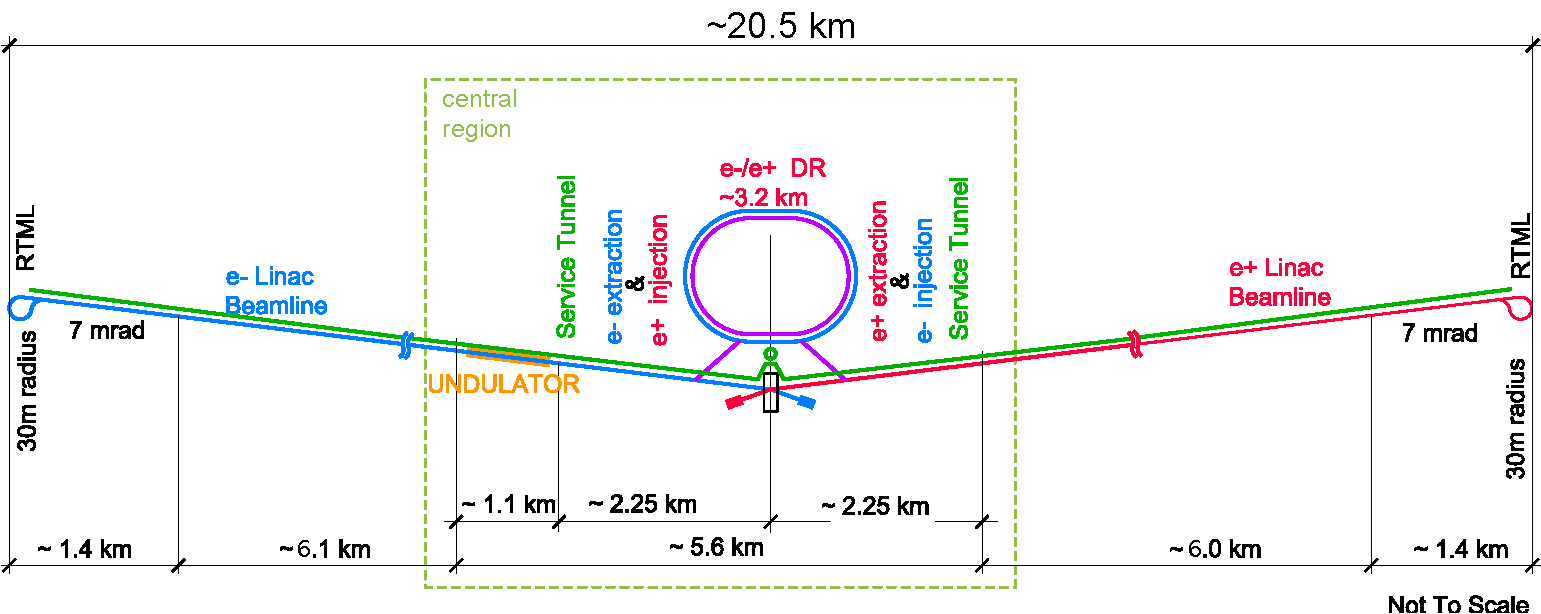
\includegraphics[width=\hsize]{figures/TDR-machine-layout-cartoon-staged.pdf}
\caption{Schematic layout of the ILC in the $250\,{\mathrm{GeV}}$ staged configuration.
\label{fig_ilc-schematic}}
 \end{center}
 \end{figure}

Electrons are produced by a polarised electron gun located in the tunnel of the positron beam delivery system. A Ti:sapphire laser impinges on a photocathode with a strained GaAs/GaAsP superlattice structure, which will provide  $90\,\%$, electron polarisation at the source, resulting in $80\,\%$ polarisation at the interaction point. The design is based on the electron source of the SLAC accelerator. 

Two concepts for positron production are considered:

The baseline solution employs superconducting helical undulators at the end of the electron main linac producing circularly polarised photons, which are converted in rotating titanium target to  positrons with a $30\,\%$ longitudinal polarisation.
This positron production scheme requires a fully commissioned electron linac delivering a beam close to $125\,{\mathrm{GeV}}$, which is a concern for commissioning and operation. 
%The main technical challenges of this concept are the target and the photon dump. 
%In addition, the undulator photon flux rapidly falls for electron energies below $125\,{\mathrm{GeV}}$, which is a concern for commissioning and operation.  
An alternative design, the electron driven source, utilises a dedicated S-band electron accelerator to provide a $3\,{\mathrm{GeV}}$ beam that is used to produce electrons.
% on a rotating titanium target. 
%Electrons are produced over a timespan of $66\,{\mathrm{ms}}$, reducing the target heat load and the necessary rotation speed.
%Technical challenges for this concept are radiation in the capture device and beam loading in the first accelerating cavities. 
This source would not provide positron polarisation,
but offer advantages for operation at lower electron beam energies and commissioning.
% as its operation is independent  from the main linac electron beam, operation at lower electron beam energies is possible and commissioning can begin in parallel to electron source commissioning.

Electrons and positrons are injected at $5\,{\mathrm{GeV}}$ into the centrally placed $3.2\,{\mathrm{km}}$ long damping ring complex, where their emittance is reduced to $2\,{\mathrm{pm}}$ ($5\,{\mathrm{\mu m}}$) in the horizontal (vertical) plane within $200\,{\mathrm{ms}}$. 
These emittance numbers are well in line with the performance of today's storage rings for advanced light sources.
To achieve the necessary damping time constant, the damping ring is equipped with $54$ superconducting wigglers. 

The damped beams are transported to the beginning of the main accelerator by two low emittance beam transport lines. Two bunch compressor stages at $5$ and $15\,{\mathrm{GeV}}$ reduce the longitudinal bunch length to $300\,{\mathrm{\mu m}}$ before the beams are accelerated to $125\,{\mathrm{GeV}}$ in the two main linacs.

The main linacs accelerate the beams in superconducting cavities made of niobium, operating at $1.3\,{\mathrm{GHz}}$ frequency and a temperature of $2.0\,{\mathrm{K}}$. 
Each cavity has $9$ cells and is $1.25\,{\mathrm{m}}$ long. The mean accelerating gradient will be $31.5$ to $35\,{\mathrm{MV/m}}$.
Cavities are mounted in $12\,{\mathrm{m}}$ long cryomodules that house $9$ cavities or $8$ cavities plus a quadrupole unit for beam focusing. 
The cryomodules provide cooling and thermal shielding to the cavities and contain all necessary pipes for fluid and gaseous helium at various temperatures, so that no separate helium transport line is necessary.
Cryomodules of this type have been in continuous operation since 2000 in the TESLA Test Facility (TTF, now FLASH) at DESY,  proving their long-term stability. 
Since September 2017, the European X-FEL at DESY has been in operation, utilizing 97 of these cryo modules. 
Cost and performance estimates for the ILC cryomodules are based on the experience from these facilities, and thus can be regarded with high confidence. 

The radiofrequency (RF) power for the cavities is generated by commercially available $10\,{\mathrm{MW}}$ klystrons with an efficiency of $65\,\%$. 
The pulse modulators will be use a new, modular and cost-effective semiconductor design \jim{developed} at SLAC, the MARX modulator.

The cryogenic system design foresees six cryo plants for the main linacs with a size similar to the plants for one LHC octant; 
two smaller plants would supply the central region including the preaccelerators of the sources and the damping rings. 

Finally, the beam delivery system focuses the beams to the required size of $516\,{\mathrm{\mu m}} \times 7.7\,{\mathrm{nm}} $. 
A feedback system, which profits from the relatively long inter bunch separation of $554\,{\mathrm{ns}}$, ensures the necessary beam stability. 
The necessary nano-beam technology has been tested at the Accelerator Test Facility 2 (ATF-2) at KEK.


The TDR baseline design was for a centre-of-mass energy of $\sqrt{s}=500\,{\mathrm{GeV}}$, upgradeable to a final energy of $1\,{\mathrm{TeV}}$.
After the discovery of the Higgs boson in 2013 interest grew for an accelerator operating as a ``Higgs factory'' at $\sqrt{s}=250\,{\mathrm{GeV}}$, slightly above the maximum for $Zh$ production. 
The design for a $250\,{\mathrm{GeV}}$ version of the ILC has recently been presented in a  staging report by the LCC directorate~\cite{Evans:2017rvt} and was endorsed by ICFA.

The staged ILC version of the ILC  
% (in the preferred ``option A'') 
would have two main linac tunnels about half the length ($6$ instead of $11\, {\mathrm{km}}$) of the $500\,{\mathrm{GeV}}$ TDR design. 
Other systems, in particular the beam delivery system and the main dumps, would retain the dimensions of the TDR design.
Thus, the ILC250 could be upgraded to energies of $500\,{\mathrm{GeV}}$ or even $1\,{\mathrm{TeV}}$ with a reasonable effort, without extensive modifications to the central region. 
Recent studies of rock vibrations from tunnel excavation in granite rock indicate that the necessary additional main linac tunnels could be largely constructed with the ILC running, so that an energy upgrade could be realised with an interruption in data taking of a couple of years only, compatible with a smooth continuation of the physics programme.

Another upgrade option, which could come before or after an energy upgrade, is a luminosity upgrade. 
Doubling the luminosity by doubling number of bunches per pulse to $2625$ at a reduced bunch separation of $366\,{\mathrm{ns}}$ would require $50\,\%$ more klystrons and modulators and an increased cryogenic capacity. 
The damping rings would also permit an increase of the pulse repetition rate from $5$ to $10\,{\mathrm{Hz}}$. 
This would require a significant increase in cryogenic capacity, or running at a reduced gradient after an energy upgrade.
% Both paths to a luminosity increase would pose large  stress for the positron source target and probably require its redesign, which would be a significant engineering challenge, but not a cost driver.
The projections for the physics potential of the ILC250 are based on a total integrated luminosity of $2\,{\mathrm{ab}}^{-1}$, which assumes at least one luminosity upgrade.

The total project cost for the construction of the $250\,{\mathrm{GeV}}$ accelerator is estimated to be $5,260\,{\mathrm{MILCU}}$, where an ILCU (ILC Currency Unit) is defined as $1\,{\mathrm{US\$}}$ in 2012 terms, plus $17\,{\mathrm{Mh}}$ of work. 
These numbers include the cost for civil engineering and the laboratory, while costs for land acquisition are exempt, as are R\&D costs before the construction start, and costs for the detectors.
The \juan{cost is calculated} as an estimate of the median project cost, without contingency or management reserve.
The cost premium to cover the project cost with $85\,\%$ instead of $50\,\%$ confidence level (loosely speaking, the $1\,\sigma$ uncertainty of the cost estimate) has been estimated to be $23\,\%$ of the estimated cost.

The construction of the accelerator will require nine years after ground breaking, preceded by a four year preparation phase.

%%%%%%%%%%%%%%


\section{\label{sec:detectrd} The Detector R\&D effort}


\todo{ 1 page - Marc.}
\todo{At present the R\&D section is copied from the original text by  Marc from Doc2. It needs to be better adapted to Doc1 and a more natural merging/transition to the detectors section. Industrial participation, interest and motivation should also be implemented.}


The capacity to reconstruct with extreme precision the characteristics of the signal states produced at the ILC is mandatory to take advantage of the inherently accurate knowledge of the scattering conditions of the beam particles. Moreover, the relatively mild running conditions allow alleviating the constraints on radiation tolerance and read-out speed. The R\&D related to each sub-system was therefore driven by a challenging and innovative trade-off to be found between very demanding resolution (granularity) and material budget requirements on the one hand, and an acceptable speed and power consumption on the other hand. Moreover, the detector steering and read-out architectures obey specific conditions: they should be operated triggerless and designed to exploit the machine duty cycle and bunch spacing to mitigate the power consumption.
In several cases, individual performances targeted by the R\&D could have been considered as nearly achieved outside of the ILC programme, but intensive R\&D was needed to realise their combination at a level well beyond previous achievements, including detailed system integration aspects. In most cases, the R\&D was aiming at an order of magnitude improvement w.r.t. the state-of-the-art. The prototyping undertaken for each experiment sub-system had as an initial goal to provide a realistic design with reliable performance and cost evaluation of the complete detector.

Overall, the R\&D on highly segmented sub-systems composing the experimental set-up was guided by the need to reconstruct each particle composing the signal states using the so-called Particle Flow Approach (PFA). The performances demonstrated by the R\&D were transferred to the Monte-Carlo description of the experiment used to predict the achievable experimental performances for each component of the physics programme.

The R\&D was conducted by a large number of groups over many years. A wide variety of technological and design options could therefore be extensively explored. Technological alternatives were investigated for all sub-systems and were compared in terms of detection performances as well as for their cost. In most cases, these detection performances were evaluated on particle beams with system aspects directly comparable to the experiment. Some beam tests were performed inside a 2 T magnetic fi�eld in order to validate the pulsed mode concept and the associated power saving.

Each calorimeter and tracking sub-system has been prototyped extensively, from small prototypes addressing all critical elements of a given sub-system up to a complete, real scale, prototype operated on beam, sometimes in combination with prototypes of other sub-systems composing the experiment. This allowed in particular to study and mature the PFA strategy with real input.

The development of tracking and vertexing devices was governed by the need of pixellated low material budget components allowing excellent momentum resolution and displaced vertices characterization, including vertex charge, with performances exceeding typically by one order of magnitude those of existing experiments.

Two alternative approaches were investigated for the main tracker, one based on a TPC and one exploiting silicon sensors, possibly pixelated. The R\&D for the TPC addressed mainly the single point resolution and ion feedback mitigation with diferent micro-pattern read-out systems (MicroMegas, GEM, ...) and showed that the performance goals can indeed be reached, with a material budget of the end-caps not exceeding 30 \% X\jim{$_0$}. The approach relying on silicon detectors concentrated on the material budget, showing that the targeted momentum resolution was reachable despite the restricted number of detector layers allowed to mitigate multiple scattering effects. These efforts have also benefited a lot from the R\&D that has been conducted for the tracker upgrades for both ATLAS and CMS, which both rely on all-silicon tracking systems. 
\jim{The tracking layers 
envisioned for the ILC are much thinner than the LHC as a consequence of the different beam conditions.}
It was also shown that, while the performance was more than adequate in terms of momentum resolution, the tracking in dense jet environments could be improved by replacing the silicon-strip sensors with a large-area pixelated tracker. 

The R\&D for the vertex detector explored the potential of several thin highly granular pixel technologies (CMOS, DEPFET, FPCCD, SoI, ...) which could off�er the projected spatial resolution and material budget. Intensive efforts were invested in read-out systems allowing to cope with the hit density induced by the beam related background, resulting in performances depending on the technology and the read-out architecture.The concept of double-sided layers was also investigated with some technologies and established up to the level of being operated near an e+e− interaction point.

A significant part of the R\&D eff�ort for the ILC detector concentrated on calorimetry, which required strategies promoting very compact and high granularity detection technologies connected to very low average power read-out micro-circuits complying with power pulsing. Major issues were addressed within the CALICE collaboration, a consortium composed of more than 300 members coming from more than 50 institutes.

The R\&D for the EM calorimeter concentrated on optimized and cost effective sensor systems, on the designs of a low power, pulsed, integrated readout electronics and an effective thermal management and calibration strategy, and on including a mechanical concept which combines large stability with minimal dead zones. A SiW based real size prototype was constructed and tested extensively on particle beams. The development of a more cost-effective technological solution, based on a scintillator and photo-multiplier matrix was also realised and some of its performances compared to those of the SiW concept.

The HCAL prototyping was governed by the need for an efficient and precise reconstruction of neutral hadron showers. Combined with stainless steel as conversion material, two read-out options were developed, one combining scintillator tiles with silicon photo-sensors read out with analog electronics, and an alternative approach based on gaseous devices (e.g. RPC) with higher segmentation but with signal encoding on one or two bits only.

The relative merits of the diff�erent ECAL and HCAL options were in particular evaluated using combined test beam campaigns providing common data which were processed with PFA software which it allowed developing and assessing at the same time. The possibility to achieve the targeted energy and topology resolutions was demonstrated even when operated in power pulsed mode.

Substantial effort was invested in developing technological solutions for the very forward calorimeters designed for robust electron and photon measurements used for integrated luminosity measurements and for bunch-to-bunch machine parameter monitoring. Satisfactory performances, including a radiation tolerance to 1 MGy, were obtained with tungsten absorber layers alternated with GaAs sensor planes read out with dedicated electronics featuring a dual gain charge amplifier providing a fast feedback for beam tuning.

Summarizing, despite constrained \jim{financial} conditions, the proof of principle underlying each prominent sub-system of an experiment at the ILC has been completed. Most of the detector prototypes fabricated and tested allow extrapolating to the full detector performance and cost. Some technologies and detector concepts developed for the ILC have influenced existing experiments in their construction of upgrade phase, which in turn provide a full size validation of technological approaches first developed for the ILC. Further studies addressing system integration aspects are however still needed for some subsystems. The optimization of the complete experimental design, though quite advanced, also still requires additional studies. The few years foreseen to finalize the decision and procedure of constructing the ILC will provide the necessary time to make the most appropriate technological choices for each sub-system and to complete the full R\&D programme in due time. \todo{this paragraph should be included in the discussion section ?}


%%%%%%%%%%%%%%


\section{\label{sec:detect} The ILC detectors}

\todo{ 2 pages - Ties, Andy}

\todo{introductory paragraph is needed to connect with the R\&D section and giving continuity to the whole programme: detector designed being the consequence of the Machine conditions, physics requirements and detector R\&D progress.}

The science at the ILC drives the requirements on detectors. The main factors are:


\begin{figure}[tb]
 %\epsfysize=9.0cm
 \begin{center}
 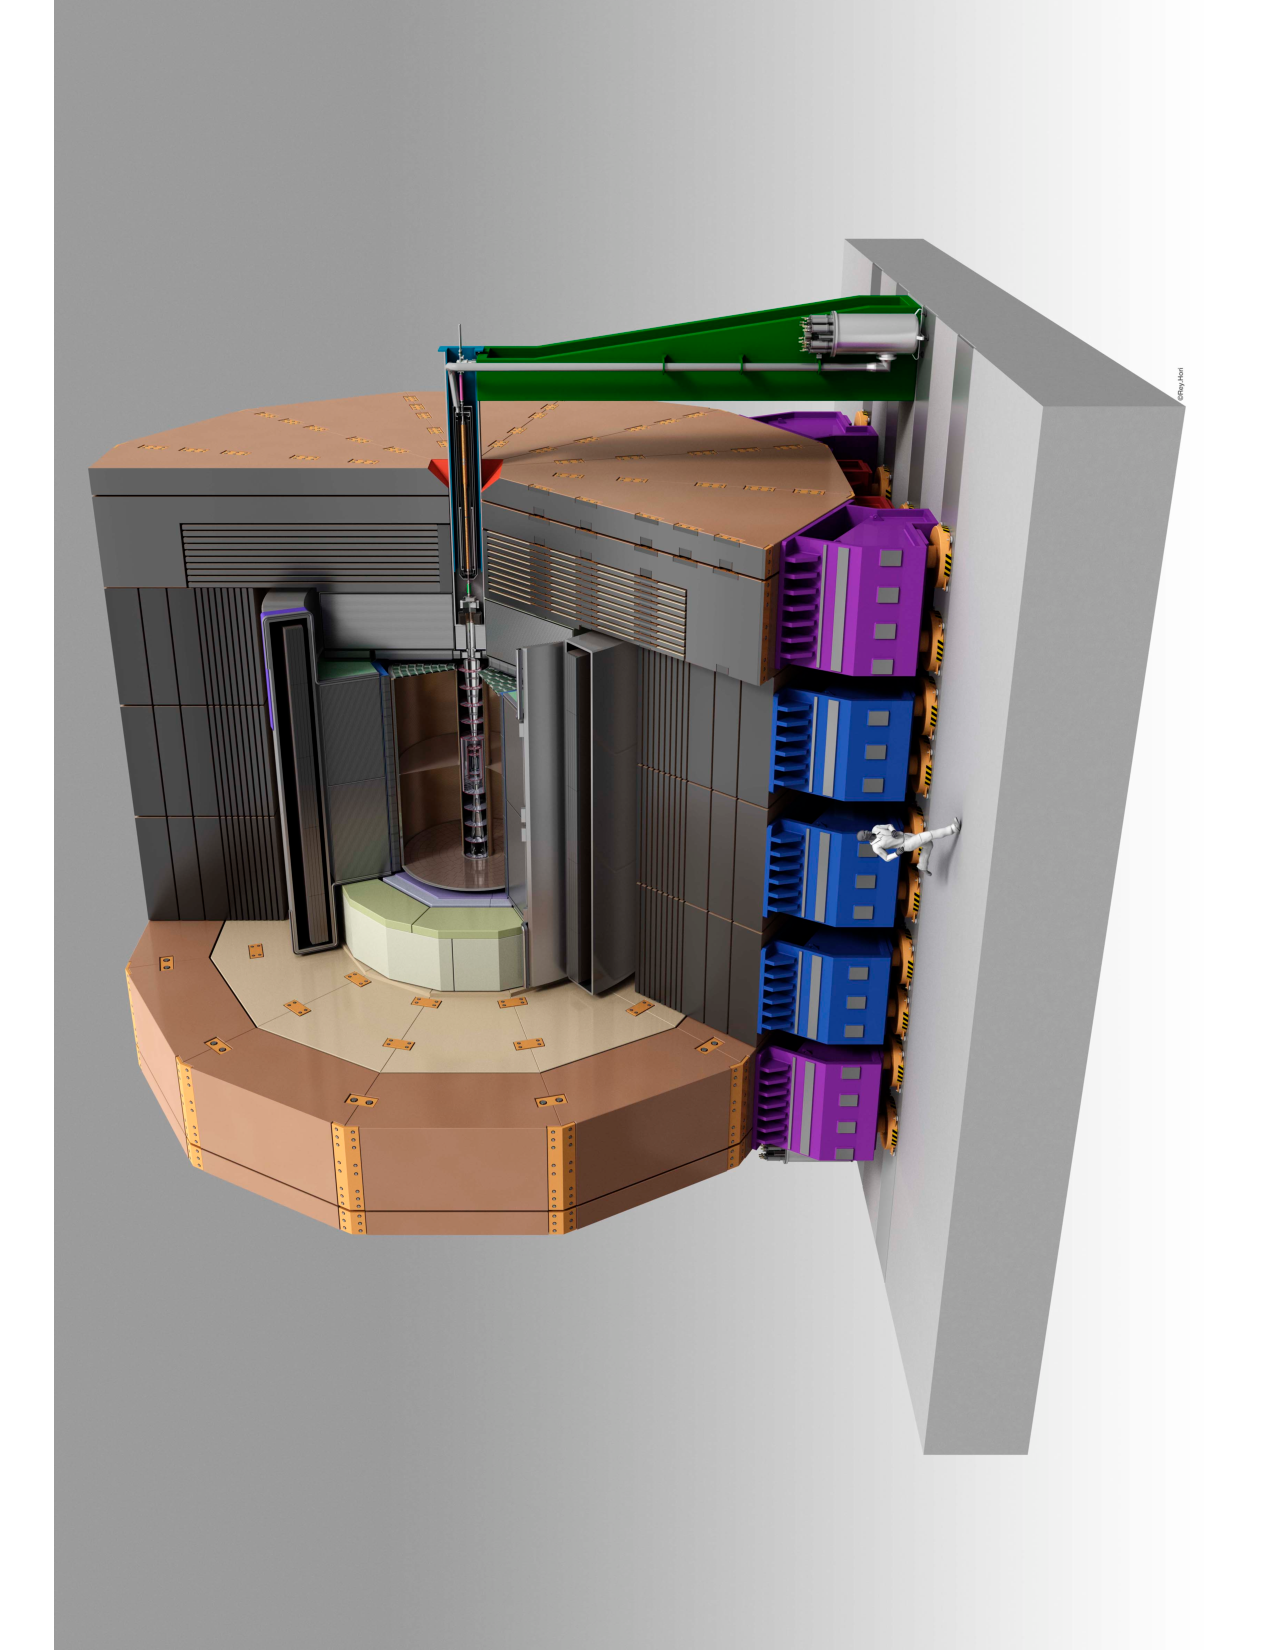
\includegraphics[width=0.8\hsize,angle=-90]{figures/ILD.pdf}
\caption{The ILD detector concept.
\label{fig_ild}}
 \end{center}
 \end{figure}
 
 
\begin{itemize}
 \item The detector has to have an excellent track momentum
   resolution. The benchmark reaction here is the analysis 
of the di-lepton mass in the process $HZ \to H \ell^+
\ell^-$. This reaction allows the reconstruction of the 
Higgs mass independent of its decay mode via the 
reconstruction of the lepton recoil spectrum. In order that 
the momentum resolution of the detector does not limit 
the mass resolution achievable for the recoiling lepton 
system, stringent momentum resolution requirements have to be met. 
\item The reconstruction of the flavour of the final state can 
often be done best with the help of lifetime information of the 
decaying particles. For this, very powerful vertex detectors 
are needed. This is particularly important 
in the Higgs sector, where -- at least for light Higgs bosons -- 
a large fraction of the Higgs decays has bottom 
quarks in the final state. Many other physics signatures will 
produce complex final states with bottom or charm quarks as well. 
A supreme vertex detector therefore is needed to reconstruct these 
long lived particles with excellent resolution. 
\item The overall event is best reconstructed with the 
particle flow measurement. The particle flow technique combines 
the information from the tracking systems and from the 
calorimetric systems in an attempt to reconstruct the 
energy and the direction of all charged and 
neutral particles in the event. To minimize overlaps between 
neighboring particles, and to maximize the probability to 
correctly combine tracking and calorimeter information, 
excellent calorimeters are needed with very high granularity. 
\item Many physics signatures predict some undetectable particles, 
which escape from the detector. They can only be reconstructed by 
measuring the missing energy in the event. This requires 
that the detector is as hermetic as possible, to 
minimize the amount of energy that can escape detection. 
Particular care has to be given to the region surrounding the 
beampipe in the forward direction. 
\end{itemize}

Compared to the last large scale detector project in particle physics, the construction and upgrade of the LHC detectors, the emphasis for linear collider detector is shifted towards ultimate precision. This requires \jim{detector technologies} which are driven towards ultimate precision, and this requires a minimisation of dead material in the detector, at an unprecedented level. This also requires a management and control of services and in particular a thermal management of the detector concept. Significant technological R\&D was needed to demonstrate the feasibility, and is, in fact, still ongoing, as \jim{is} discussed in the \jim{last} section.  


\begin{figure}[tb]
 %\epsfysize=9.0cm
 \begin{center}
 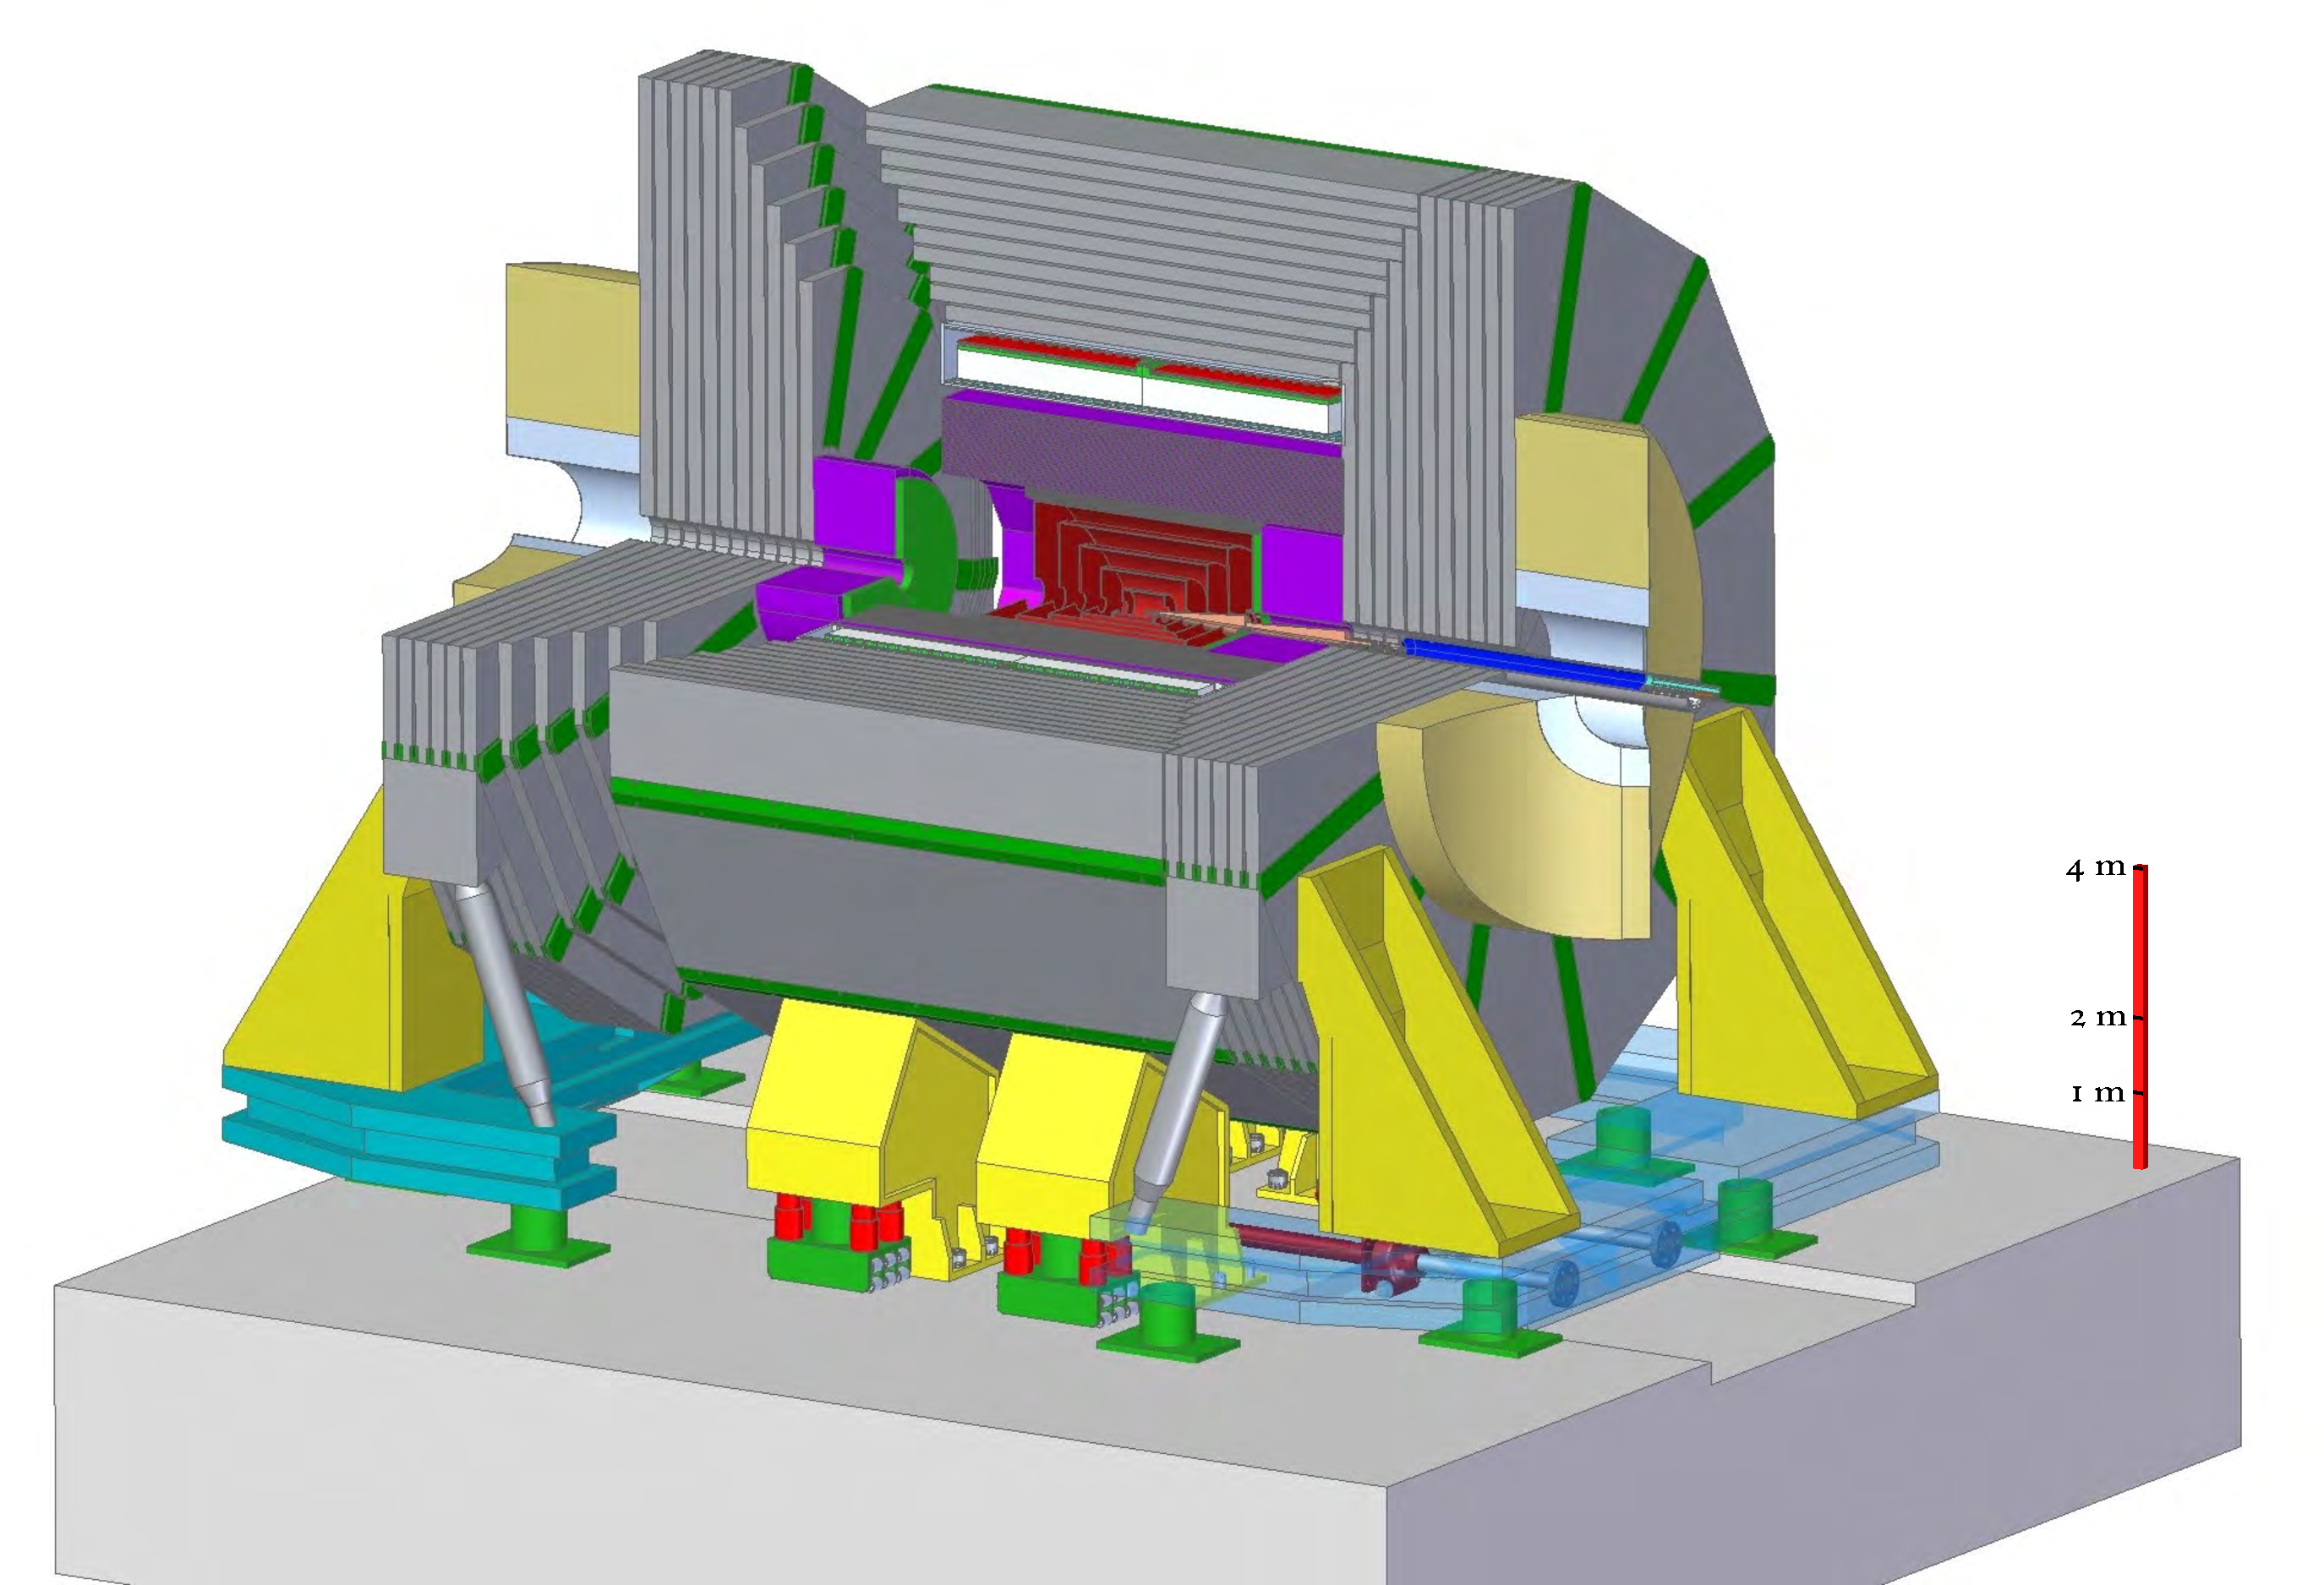
\includegraphics[width=\hsize]{figures/SiD.pdf}
\caption{The SiD detector concept.
\label{fig_sid}}
 \end{center}
 \end{figure}


Over the last decade two detector concepts have emerged from the discussions in the community. Both are based on the assumption that particle flow reconstruction plays a central role in the event reconstruction. Both therefore have highly granular calorimeters, placed inside the coil which is providing the central magnetic field. Both have excellent trackers and vertexing systems. The two approaches differ in the choice of tracker technology, and in the approach taken to maximize the overall precision of the event reconstruction. ILD \jim{(\Fig{fig_ild}) } has chosen a gaseous central tracker, a time projection chamber, combined with silicon detectors inside and outside the TPC. SiD \jim{(\Fig{fig_sid}) } relies on an all silicon solution, similar to the LHC detectors, \jim{although with
much thinner silicon layers}. ILD tries to optimize the particle flow resolution by making the detector large, thus separating charged and neutral particles. SiD keeps the detector more compact, and compensates the reduced particle separation at the position of the calorimeters by using a higher central magnetic field. Both approaches have demonstrated excellent performance, meeting or even exceeding the performance requirements. 



For both detector concepts, communities have found themselves and pre-collaborations have formed. These organizations have over the last ten years or so pushed both concepts to a remarkable level of maturity, and have, in close interaction with the different groups performing detector R\&D from around the world, demonstrated the feasibility to build and operate such high precision detectors. 

European groups have played a central role in these efforts. The ILD concept group is formed from some 70 groups from around the world, with more than half coming from Europe. The SiD collaboration has a strong basis in the Americas, but also relies on significant participation from European groups. Major contributions to the development of all sub-systems have come from Europe. Significant technological breakthroughs for example in the area of highly granular calorimeter are strongly driven by European groups. 

An important aspect of the detector concept work has been in addition to the development and demonstration of the technology the integration of the detector into the collider and into the proposed site. The location of the experiment in an earth-quake prone area poses challenges which have been addressed through R\&D on detector stability, support and service. The scheme to operate two detectors in one interaction region, the so called push-pull scheme, has no example and needed significant engineering work to demonstrate its feasibility. With strong support from particle physics laboratories in Europe, in  particular DESY and CERN, many of the most relevant questions could be answered and the feasibility of the approach could be demonstrated at least in principle. 


\section{\label{sec:soft}Software and Computing}

\todo{ [1 page - Frank G. and Akiya
Description of ILC software and computing requirements] }

The excellent and unprecedented detector resolution of the two proposed ILC detector concepts described
in the previous section is of course crucial for meeting the ambitious physics goals
defined for the ILC programme. However achieving the ultimate physics performance is only possible if it
is complemented with powerful software tools at all levels of the data processing. This starts with the
detailed detector description for simulation, followed by sophisticated event reconstruction algorithms
and is completed with high-performance and easy to use tools for physics analyses.
For over a decade the ILC community has developed and improved its software ecosystem, called \emph{iLCSoft}.
At the heart of \emph{iLCSoft} are the common event data model LCIO, the Marlin application framework and the
DD4hep detector description toolkit. These tools provide the basis for almost all linear collider related
studies carried over the years, including those for CLIC and also recently for CEPC.
From the start a strong focus has been put on developing flexible and generic tools that can easily be applied
to other experiments or new detector concepts. This approach of developing common tools wherever possible
has helped a lot in leveraging the limited manpower and putting the focus on the algorithm development that
is crucial for the physics performance. Recent developments evolving around the Hep Software Foundation are
now following a similar strategy, also for the LHC experiments.
For both detectors there are simulation models with realistic descriptions of the detector technologies,
the dead material, gaps, imperfections, as well as detector services. These models have been used for large
scale Monte Carlo productions and physics analyses for the TDR and more recent detector optimization
campaigns. Based on these studies, we already now have a rather good understanding of the expected
detector performance and physics reach of the ILC.
The development of \emph{iLCSoft} is a truly international activity, where European groups, in particular DESY and
CERN have played a leading role and should continue to do so, if the ILC will be approved. In this case
a strong focus will be on adapting the software tools for modern hardware architectures and continue to
further improve the computing and physics performance of the algorithms.


  
An initial computing concept for the ILC, including a first estimate of the required resources, has been developed by the LCC Software and Computing Group.
This concepts follows in general terms that of other ongoing experiments at the LHC and Belle-2 with a strong on-site computing center, complemented with large
Grid-based computing resources distributed around the world. However, due to he much lower event rates at the ILC, compared to the LHC, we will be
able to run in an un-triggered mode where collision data from every bunch crossing will be recorded. At the experiment site we require only limited computing
resources for online monitoring, QA and data buffering capabilities for a few days. Prompt reconstruction, event building and filtering of the interesting collisions
will be performed at the main ILC campus, resulting in a data reduction of around 97\%. The reminder of the data will be distributed to major participating Grid sites
in the world for further skimming and final redistributed for physics analysis.
Based on detailed physics and background simulations we estimate the total raw data rate of the ILC to be $\sim$1.5GB/s, resulting in about 10-15 PB/y storage needs.
The estimated computing power that will be needed for simulation, reconstruction and analysis will be around 200-300 kHepSpec06.
Given that these numbers are already smaller than what is needed by the LHC experiments today and an expected annual increase of 15\% and 25\% for storage and CPU
respectively at flat budget, we expect the overall computing costs for the ILC to be more than an order of magnitude small than those for the LHC.

\section{\label{sec:discuss}Discussion}

\todo{ 1 page - Keisuke, Jim and Juan
Discussion of HEP community interest and support, political progress, plan for international realization, weight on ILC250 for searches and discovery potential, opportunity for young generations, maturity of the technology -detectors and accelerator-, reliability on cost estimates, etc..}

\section{\label{sec:sum}Summary \& Conclusion} 

\todo{ 1 page }

%\bibliographystyle{utphysmod}
\bibliography{ILC-ESU-refs}


\end{document}
%
% ****** End of file apssamp.tex ******
